% !TeX root = ../../Thesis.tex
\chapter{Introduction}
\label{chp:introduction}
The material presented in this thesis represents kinetic simulations of laser-plasma interactions (\acrshort{LPI}) relevant to direct-drive inertial confinement fusion (\acrshort{ICF}). In this introductory chapter, an overview of the goals of, and approaches to, inertial confinement fusion is given; including specific details of the `shock-ignition' (\acrshort{SI}) ICF scheme. We then review the previous work concerning laser-plasma interactions in direct-drive ICF, and motivate the use of kinetic modelling throughout this thesis. Finally, we offer an outline of the rest of the thesis.

\section{Inertial Confinement Fusion}
The basic concept of inertial confinement fusion (\acrshort{ICF}) is based on the Ulam-Teller design for a thermonuclear weapon (H-bomb), which uses radiation to compress thermonuclear fuel to the point where it undergoes nuclear fusion \citep{SpanishHistoryOfICF}.  Nuclear fusion is the process by which two light atomic nuclei combine to form a new, heavier, nucleus and release energy proportional to the mass gap as kinetic energy of the fusion products. The reaction of choice in the thermonuclear weapon, and in most modern ICF designs, is deuterium-tritium (\acrshort{DT}) fusion. Equation \ref{eq:DTfusion} shows the reaction first in the most commonly-presented formula, and then explicitly in terms of the ions and their neutron (superscript) and proton (subscript) numbers.

\begin{equation}\label{eq:DTfusion}
\begin{aligned}
	\text{D} + \text{T} &\longrightarrow \text{He}^4 + \text{n} + 17.6 \si{\mega\electronvolt}\\
	\text{H}^2_1 + \text{H}^3_1 &\longrightarrow \text{He}^4_2 (3.5\si{\mega\electronvolt}) + \text{n}^1_0 (14.1\si{\mega\electronvolt}).
\end{aligned}
\end{equation}
In order for a fusion reaction to be usable on earth, we require that it satisfies certain criteria: uses the lightest possible elements; reaction occurs at `reasonable' temperatures (on the order of $10 \si{\kilo\eV}$); reactants (fuel) are obtainable. Figure \ref{fig:crossSection} shows that the \acrshort{DT} reaction has the largest cross section / highest thermal reactivity of the several reactions which satisfy the above conditions.

\begin{figure}
 \centering
 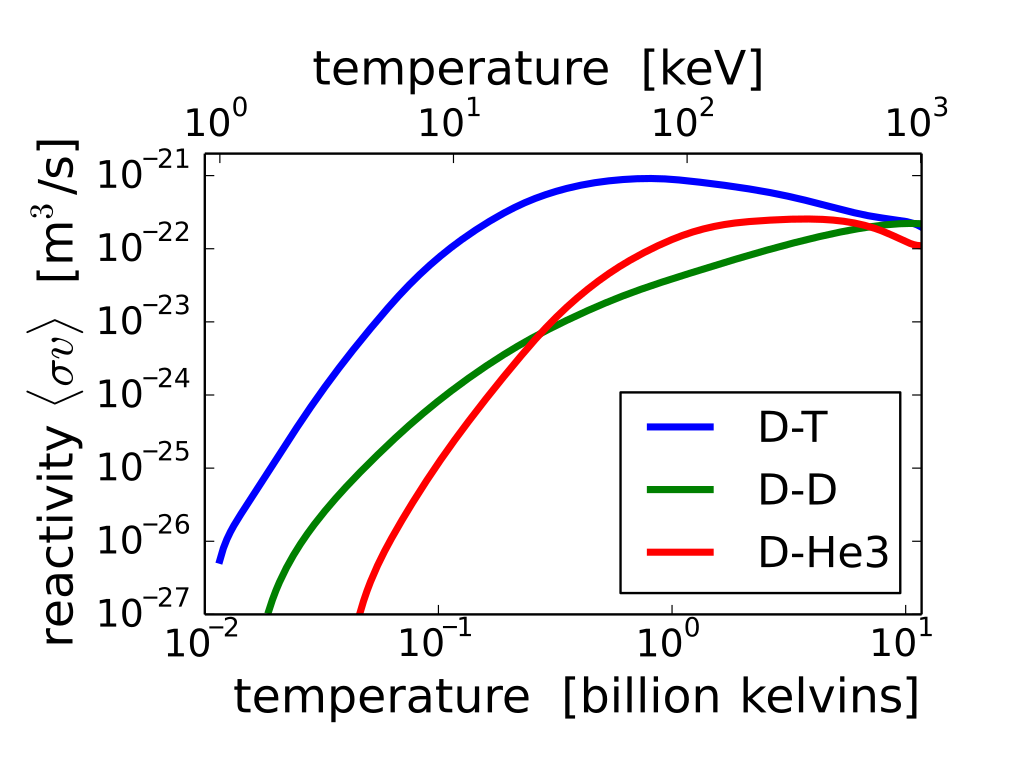
\includegraphics[width=0.7\columnwidth]{Chapters/C1_Introduction/crossSection.png}
 \caption{source: Dstrozzi, CC BY 2.5, via Wikimedia Commons, \url{https://commons.wikimedia.org/wiki/File:Fusion_rxnrate.svg}} \label{fig:crossSection}
\end{figure}

\subsection{Radiation implosion}
In the thermonuclear weapon, the radiation source is a fission bomb, which detonates and reaches very high temperatures, producing thermal x-rays which are channelled to compress the thermonuclear fuel.

\subsection{Aims of ICF research}

The aims of ICF research programmes have changed throughout history.

A recent paper by \citet{Nicholas2021} suggests that fusion energy (whether through ICF or magnetically confined fusion) will not be ready in time to act as a replacement for fossil fuels, which must be removed from the energy mix by BLAH if we are to avoid the worst impacts of catastrophic climate change. They assume that, by the second half of the 21st century, renewable energies such as wind and solar will pwoer most of the grid. However, the intermittent nature of these mechanisms will leave a gap in the energy market for a carbon-free source of baseload energy \citep{Nicholas2021}. In order for fusion energy to be a good choice for filling this gap it must be able to demonstrate its superiority over traditional nuclear fission power generation. This may include showing its better performance in terms of: waste production; ease of proliferation; and resource supply. In light of this analysis, the work presented in this thesis may never directly contribute to usable, or desirable, ICF energy-generation schemes.

\subsection{Direct and indirect drive ICF}

\subsection{Shock-ignition}
Having covered the differences between \acrshort{LDD} and  \citep{Ribeyre2009} we come to the ignition scheme considered in this thesis, shock ignition. This is a directly-driven central ignition scheme boosted by a strong shock.

\section{Previous work}
\subsection{Laser-plasma interactions in shock-ignition}
\subsection{Simulations}
\subsubsection{Kinetic models}
\subsubsection{Fluid models with kinetic effects}
Basically it's interesting that you can put some of these effects into a fluid model, such as here \citep{Tran2020}
\subsection{Experiments}

\subsection{Why PIC in this thesis?}
Question: doesn't PIC suck for predicting experimental observables? 

\section{Thesis Outline}
Gonna write these things

%\bibliographystyle{plainnat}
%\bibliography{Chapters/C1_Introduction/Introduction}
